% =====================================================================
% Figure: patterns of A-level economics provision among switcher schools
% Self-contained apart from: tikz, pgfplots, pgfplotstable, compat=1.18
% Numbers pasted from seq_patterns.txt and seq_types.txt
% =====================================================================
\begin{figure}[p]
\caption{Patterns of A-level economics provision among switcher schools}
\setlength{\parskip}{0pt}

% ---- styling, local to this figure ----
\definecolor{cOffer}{HTML}{2C5F8A}
\definecolor{cNoOffer}{HTML}{DCE3EA}
\definecolor{cBar}{HTML}{2C5F8A}

% one cell of the pattern grid
\newcommand{\seqcell}[3]{%
  % #1 = column (1-based), #2 = row (1-based), #3 = 0 or 1
  \ifnum#3=1\relax\def\cellcol{cOffer}\else\def\cellcol{cNoOffer}\fi
  \fill[\cellcol, rounded corners=0.4pt]
    ({(#1-1)*0.62}, {-(#2-1)*0.46}) rectangle
    ({(#1-1)*0.62+0.54}, {-(#2-1)*0.46-0.36});
}

% one row: #1 = row number, #2 = comma list of 0/1, #3 = school count
\newcommand{\seqrow}[3]{%
  \foreach \v [count=\c] in {#2} {\seqcell{\c}{#1}{\v}}%
  \node[anchor=west, font=\footnotesize]
    at ({8*0.62+0.10}, {-(#1-1)*0.46-0.18}) {#3};
}

\centerline{%
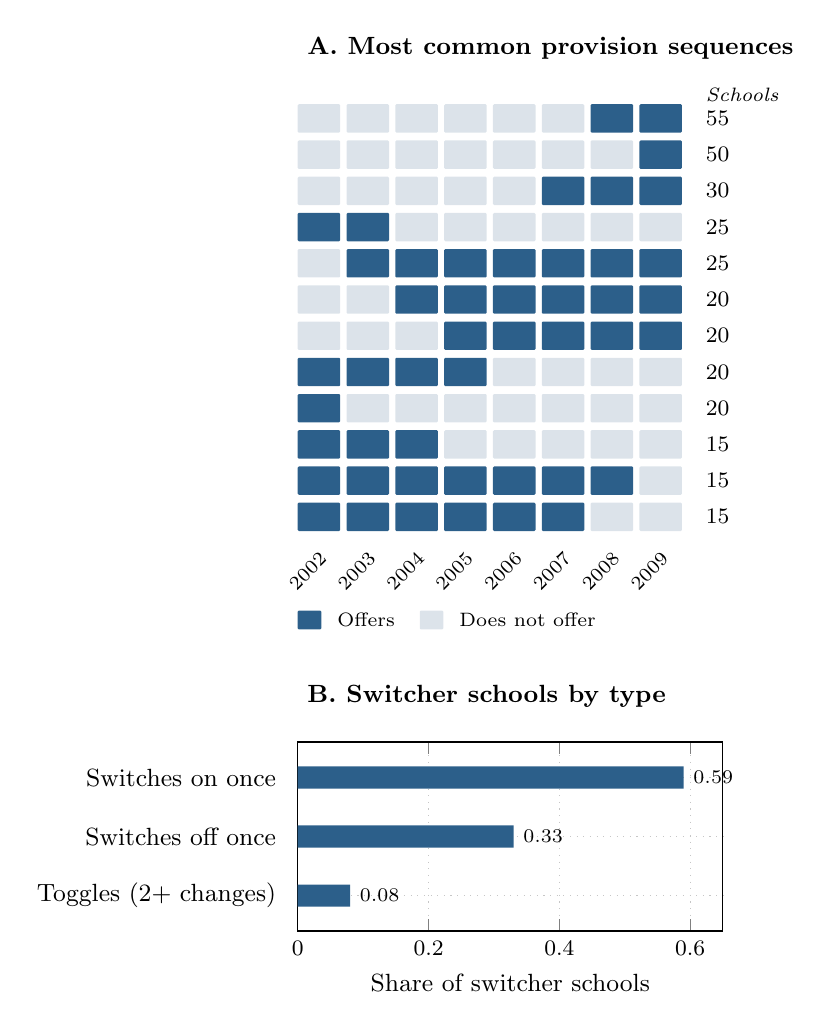
\begin{tikzpicture}

% =====================================================================
% A. Most common provision sequences
% =====================================================================
\begin{scope}[shift={(0,0)}]

\node[anchor=south west, font=\bfseries\small] at (0,0.45)
  {A. Most common provision sequences};

% ---- paste from seq_patterns.txt ----
% cells = one digit per cohort (1 = offers, 0 = does not)
% n     = number of switcher schools with this sequence
\seqrow{1}{0,0,0,0,0,0,1,1}{55}
\seqrow{2}{0,0,0,0,0,0,0,1}{50}
\seqrow{3}{0,0,0,0,0,1,1,1}{30}
\seqrow{4}{1,1,0,0,0,0,0,0}{25}
\seqrow{5}{0,1,1,1,1,1,1,1}{25}
\seqrow{6}{0,0,1,1,1,1,1,1}{20}
\seqrow{7}{0,0,0,1,1,1,1,1}{20}
\seqrow{8}{1,1,1,1,0,0,0,0}{20}
\seqrow{9}{1,0,0,0,0,0,0,0}{20}
\seqrow{10}{1,1,1,0,0,0,0,0}{15}
\seqrow{11}{1,1,1,1,1,1,1,0}{15}
\seqrow{12}{1,1,1,1,1,1,0,0}{15}
% ----------------------------------------

% cohort axis
\foreach \c [count=\i] in {2002,2003,2004,2005,2006,2007,2008,2009} {
  \node[font=\scriptsize, anchor=north, rotate=45, anchor=north east]
    at ({(\i-1)*0.62+0.27}, {-12*0.46+0.02}) {\c};
}
\node[anchor=west, font=\scriptsize\itshape]
  at ({8*0.62+0.10}, {0.12}) {Schools};

% key
\fill[cOffer, rounded corners=0.4pt] (0,{-12*0.46-1.15})
   rectangle +(0.30,0.24);
\node[anchor=west, font=\scriptsize] at (0.38,{-12*0.46-1.03}) {Offers};
\fill[cNoOffer, rounded corners=0.4pt] (1.55,{-12*0.46-1.15})
   rectangle +(0.30,0.24);
\node[anchor=west, font=\scriptsize] at (1.93,{-12*0.46-1.03})
   {Does not offer};

\end{scope}

% =====================================================================
% B. Switcher schools by type of change
% =====================================================================
\begin{axis}[
    name=panelB,
    at={(0cm,-8.1cm)}, anchor=north west,
    scale only axis,
    width=5.4cm, height=2.4cm,
    title={B. Switcher schools by type},
    title style={at={(0,1)}, anchor=south west, yshift=3pt,
                 font=\bfseries\small},
    xbar,
    bar width=8pt,
    xmin=0, xmax=0.65,
    xtick={0,0.2,0.4,0.6},
    xticklabel style={/pgf/number format/fixed, font=\footnotesize},
    xlabel={Share of switcher schools},
    xlabel style={font=\small},
    y dir=reverse,
    symbolic y coords={SwitchOn,SwitchOff,Toggle},
    ytick={SwitchOn,SwitchOff,Toggle},
    yticklabels={{Switches on once},{Switches off once},
                 {Toggles (2+ changes)}},
    yticklabel style={font=\small},
    ytick style={draw=none},
    enlarge y limits=0.30,
    grid=major,
    grid style={dotted, gray!45},
    nodes near coords,
    nodes near coords style={font=\scriptsize,
                             /pgf/number format/fixed,
                             /pgf/number format/precision=2},
]

% ---- paste from seq_types.txt ----
\addplot[fill=cBar, draw=none] coordinates {
    (0.59,SwitchOn)
    (0.33,SwitchOff)
    (0.08,Toggle)
};
% ----------------------------------------

\end{axis}

\end{tikzpicture}}

\label{fig:sequence}
\begin{singlespace}
\fignote{Notes: Restricted to schools whose A-level economics provision
changes at least once across the 2002--2009 GCSE cohorts, and which are
observed in every cohort. Panel A shows the twelve most common provision
sequences, one row per sequence and one cell per cohort; shaded cells
indicate cohorts to which the school offered A-level economics. The
right-hand column gives the number of schools following each sequence.
Sequences followed by fewer than ten schools are suppressed. Panel B
classifies all switcher schools by whether provision changes once or more
than once.}
\end{singlespace}
\end{figure}
